\section{moeo\-Random\-Select$<$ MOEOT $>$ Class Template Reference}
\label{classmoeoRandomSelect}\index{moeoRandomSelect@{moeoRandomSelect}}
Selection strategy that selects only one element randomly from a whole population.  


{\tt \#include $<$moeo\-Random\-Select.h$>$}

Inheritance diagram for moeo\-Random\-Select$<$ MOEOT $>$::\begin{figure}[H]
\begin{center}
\leavevmode
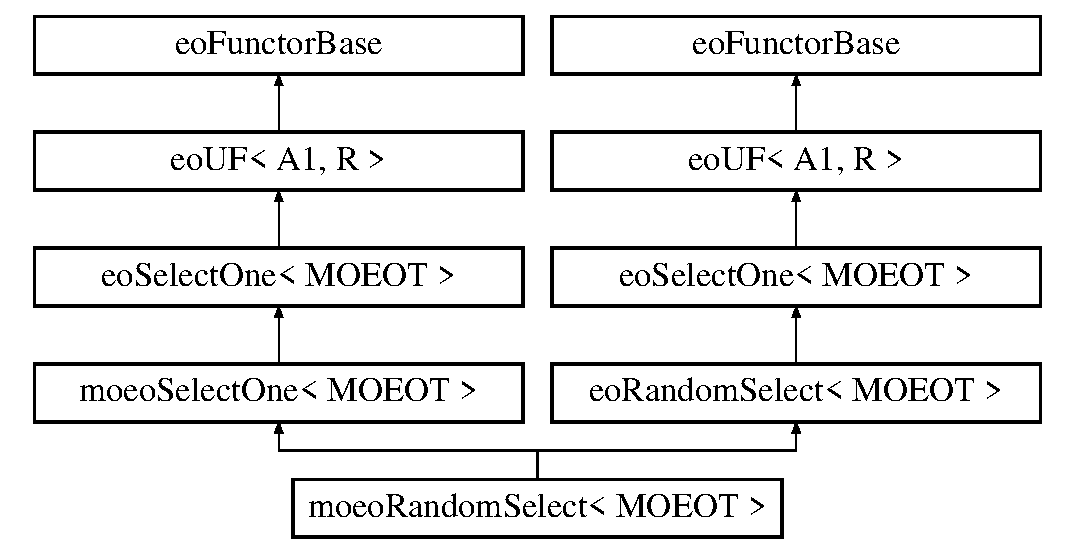
\includegraphics[height=5cm]{classmoeoRandomSelect}
\end{center}
\end{figure}
\subsection*{Public Member Functions}
\begin{CompactItemize}
\item 
{\bf moeo\-Random\-Select} ()\label{classmoeoRandomSelect_209022add1e1750f28497dfe637bb5dc}

\begin{CompactList}\small\item\em Ctor. \item\end{CompactList}\item 
const MOEOT \& {\bf operator()} (const {\bf eo\-Pop}$<$ MOEOT $>$ \&\_\-pop)\label{classmoeoRandomSelect_96dbd0832ad677090ef79ff3867d7af9}

\begin{CompactList}\small\item\em Return one individual at random by using an {\bf eo\-Random\-Select}. \item\end{CompactList}\end{CompactItemize}


\subsection{Detailed Description}
\subsubsection*{template$<$class MOEOT$>$ class moeo\-Random\-Select$<$ MOEOT $>$}

Selection strategy that selects only one element randomly from a whole population. 



Definition at line 22 of file moeo\-Random\-Select.h.

The documentation for this class was generated from the following file:\begin{CompactItemize}
\item 
moeo\-Random\-Select.h\end{CompactItemize}
